\documentclass[]{article}
\usepackage{lmodern}
\usepackage{amssymb,amsmath}
\usepackage{ifxetex,ifluatex}
\usepackage{fixltx2e} % provides \textsubscript
\ifnum 0\ifxetex 1\fi\ifluatex 1\fi=0 % if pdftex
  \usepackage[T1]{fontenc}
  \usepackage[utf8]{inputenc}
\else % if luatex or xelatex
  \ifxetex
    \usepackage{mathspec}
    \usepackage{xltxtra,xunicode}
  \else
    \usepackage{fontspec}
  \fi
  \defaultfontfeatures{Mapping=tex-text,Scale=MatchLowercase}
  \newcommand{\euro}{€}
\fi
% use upquote if available, for straight quotes in verbatim environments
\IfFileExists{upquote.sty}{\usepackage{upquote}}{}
% use microtype if available
\IfFileExists{microtype.sty}{%
\usepackage{microtype}
\UseMicrotypeSet[protrusion]{basicmath} % disable protrusion for tt fonts
}{}
\usepackage[margin=1in]{geometry}
\usepackage{graphicx}
\makeatletter
\def\maxwidth{\ifdim\Gin@nat@width>\linewidth\linewidth\else\Gin@nat@width\fi}
\def\maxheight{\ifdim\Gin@nat@height>\textheight\textheight\else\Gin@nat@height\fi}
\makeatother
% Scale images if necessary, so that they will not overflow the page
% margins by default, and it is still possible to overwrite the defaults
% using explicit options in \includegraphics[width, height, ...]{}
\setkeys{Gin}{width=\maxwidth,height=\maxheight,keepaspectratio}
\ifxetex
  \usepackage[setpagesize=false, % page size defined by xetex
              unicode=false, % unicode breaks when used with xetex
              xetex]{hyperref}
\else
  \usepackage[unicode=true]{hyperref}
\fi
\hypersetup{breaklinks=true,
            bookmarks=true,
            pdfauthor={Lisa MALIPHOL},
            pdftitle={Diateam: SCAD@COPS A Hybrid Network Intrusion Detection System},
            colorlinks=true,
            citecolor=blue,
            urlcolor=blue,
            linkcolor=magenta,
            pdfborder={0 0 0}}
\urlstyle{same}  % don't use monospace font for urls
\setlength{\parindent}{0pt}
\setlength{\parskip}{6pt plus 2pt minus 1pt}
\setlength{\emergencystretch}{3em}  % prevent overfull lines
\setcounter{secnumdepth}{0}

%%% Use protect on footnotes to avoid problems with footnotes in titles
\let\rmarkdownfootnote\footnote%
\def\footnote{\protect\rmarkdownfootnote}

%%% Change title format to be more compact
\usepackage{titling}
\setlength{\droptitle}{-2em}
  \title{Diateam: SCAD@COPS\\A Hybrid Network Intrusion Detection System}
  \pretitle{\vspace{\droptitle}\centering\huge}
  \posttitle{\par}
  \author{Lisa MALIPHOL}
  \preauthor{\centering\large\emph}
  \postauthor{\par}
  \predate{\centering\large\emph}
  \postdate{\par}
  \date{July 2015}




\begin{document}

\maketitle


{
\hypersetup{linkcolor=black}
\setcounter{tocdepth}{2}
\tableofcontents
}
\section{Introduction}\label{introduction}

\subsection{Project background}\label{project-background}

\subsection{Problem definition}\label{problem-definition}

\subsection{Paper organization}\label{paper-organization}

\section{SCADA Systems}\label{scada-systems}

\subsection{Terms}\label{terms}

\subsubsection{ICS}\label{ics}

\subsubsection{SCADA}\label{scada}

\subsubsection{PLC}\label{plc}

\subsubsection{RTU}\label{rtu}

\subsubsection{HMI}\label{hmi}

\subsection{Traffic characterization}\label{traffic-characterization}

\section{Protocols}\label{protocols}

\subsection{TCP}\label{tcp}

\subsection{MODBUS/TCP}\label{modbustcp}

\section{Common Attacks on SCADA}\label{common-attacks-on-scada}

\subsection{Command Injection}\label{command-injection}

\subsection{Response Injection}\label{response-injection}

\subsection{Denial of Service}\label{denial-of-service}

\section{Intrusion Detection Systems}\label{intrusion-detection-systems}

\subsection{Host IDS}\label{host-ids}

\subsection{Network IDS}\label{network-ids}

\subsubsection{Signature-based}\label{signature-based}

\subsubsection{Anomaly-based}\label{anomaly-based}

\section{Techniques of Network Intrusion
Detection}\label{techniques-of-network-intrusion-detection}

\subsection{Statistical}\label{statistical}

\subsection{Machine Learning}\label{machine-learning}

\subsection{Data Mining}\label{data-mining}

\section{Tools}\label{tools}

\subsection[Wireshark - Network Traffic Analysis
Tool]{Wireshark\footnote{\url{https://www.wireshark.org/docs/wsug_html_chunked}}
- Network Traffic Analysis
Tool}\label{wireshark1---network-traffic-analysis-tool}

Developed in 1997 by Gerald Combs originally named Ethereal, Wireshark
is now an Open Source GNU project. It is a network packet analyzer, or
``packet sniffer'', that captures and displays network packets.

Captured network packets are saved in the pcap file format and can be
dissected and parsed by Wireshark in order to analyze its contents. An
important aspect of Wireshark is that of its passive/monitoring nature
and so does not send, manipulate, or modify the data passing over the
network.

An initial packet capture file was created over simulated network
traffic using Wireshark. Using its export facilities, various files were
created for further analysis, with information such as TCP endpoints,
conversations, etc.

\subsection[TShark]{TShark\footnote{\url{https://www.wireshark.org/docs/man-pages/tshark.html}}}\label{tshark2}

Another tool from the Wireshark suite is the command-line tool similar
to tcpdump is tshark, a network protocol analyzer. In addition to
capturing packet data over a live network, it is also capable of
analyzing packets from an existing capture file. TShark was used to
parse out various pertinent variables pertaining to the Modbus/TCP
application protocol enclosed in the packet data.

\subsection{UNIX Utilities}\label{unix-utilities}

In order to further parse and transform the data, the UNIX utility tool
sed, which supports the use of regular expressions, was also used.

\subsection[R - Statistical Tool]{R - Statistical Tool\footnote{\url{http://www.r-project.org/}}}\label{r---statistical-tool3}

R is an Open Source programming language and environment used for
statistical computing and graphics. Initially developed by John Chambers
at Bell Labs as the S language in 1993, R was created as a freely
available version under the GNU project by Ross Ihaka and Robert
Gentleman at the University of Auckland, New Zealand.

Maintained by the R Development Core Team and with an active and growing
community, it provides various statistical and graphical creation
capabilities available under most operating systems, and is extensible
with numerous packages available.

\subsection{C++}\label{c}

\subsection{SQLite3}\label{sqlite3}

\subsection{MongoDB/MySQL}\label{mongodbmysql}

\section{Data Source}\label{data-source}

\section{Exploratory Data Analysis}\label{exploratory-data-analysis}

\section{Statistical
Measures/Features}\label{statistical-measuresfeatures}

\section{Architecture}\label{architecture}

\subsection{Process (Figure 1)}\label{process-figure-1}

\begin{itemize}
\itemsep1pt\parskip0pt\parsep0pt
\item
  Step 1: Data Acquisition During Normal Activity - From the IDS
  appliance, sniff the network traffic, extract and store data in a
  database.
\item
  Step 2: Statistical Analysis

  \begin{itemize}
  \itemsep1pt\parskip0pt\parsep0pt
  \item
    2.1 - Process data - Perform any transformation, filtering and data
    cleansing necessary.
  \item
    2.2 - Calculate and determine statistical measures.
  \item
    2.3 - Configure appliance with statistical parameters.
  \end{itemize}
\item
  Step 3: Detection Mode - Appliance is set to detection mode.
\end{itemize}

\subsection{Technical Architecture (Figure
2)}\label{technical-architecture-figure-2}

Figure 1 -
Process\\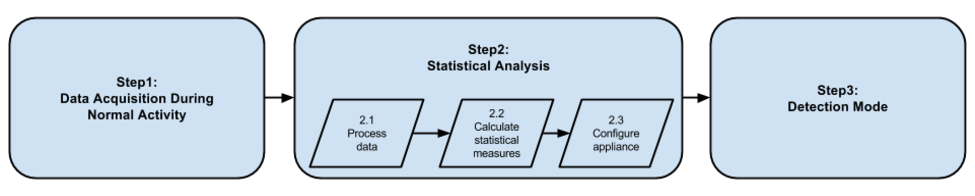
\includegraphics{reportV1_files/figure-latex/unnamed-chunk-2-1.pdf}

Figure 2 - Technical
Architecture\\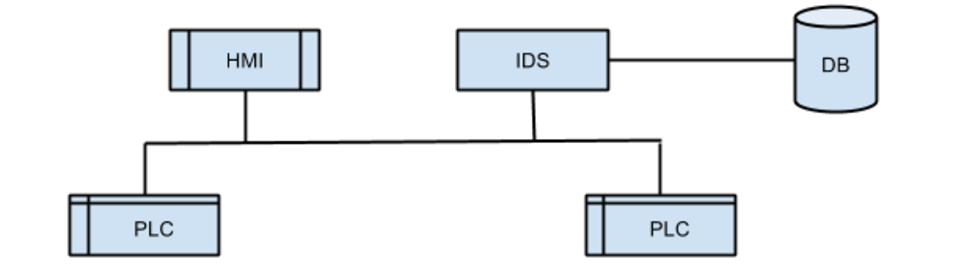
\includegraphics{reportV1_files/figure-latex/unnamed-chunk-3-1.pdf}

\section{Implementation}\label{implementation}

\section{Testing/Evaluation}\label{testingevaluation}

\section{Conclusion/Future Work}\label{conclusionfuture-work}

\section{Glossary}\label{glossary}

\section{Bibliography}\label{bibliography}

\section{Appendices}\label{appendices}

\end{document}
